\chapter{弗里德曼動力學：物質、輻射與真空能}

\lectureoverview{膨脹宇宙的運動學可以用一句話表述：物理間距隨標度因子\(a(t)\)增大。現在的問題是要決定這個函數。我們將從牛頓能量守恆導出平直空間的弗里德曼方程，先求解普通物質主導的情形，再看看為什麼輻射和真空能會帶來截然不同的宇宙演化史。}

\section{待解釋的幾何}

在固定的宇宙時刻，大尺度宇宙看起來均勻且各向同性。星系、星系團和超星系團當然是真實存在的結構，但在數億或數十億光年的尺度上，它們的分布會變得非常均勻。這種經驗規律稱為宇宙學原理。名稱本身並不會使它成為定理；這項原理的根據來自觀測。

還有第二個經驗事實。在目前的觀測精度下，大尺度空間三角形的表現如同歐幾里得三角形。拿測量足球場來類比很有幫助。如果拉緊的線構成的三角形內角和為\(180^\circ\)，這並不能證明地球整體是平的；它所顯示的是，地球的曲率半徑遠大於足球場。宇宙測量的邏輯也相同：空間可能有非常大的曲率半徑，但在可觀測區域內仍可很好地近似為平直。

作為參照的幾何是閔可夫斯基時空，
\begin{equation}
  d\tau^2=dt^2-\left(dx^2+dy^2+dz^2\right).
  \label{eq:l09-minkowski}
\end{equation}
括號內就是三維歐幾里得距離元。相較之下，在廣義相對論中，座標微分前的係數是場；它們可能隨位置和時間改變，也可能出現混合項。這些度規係數是牛頓引力場在相對論中的對應物。

\begin{figure}[H]
  \centering
  \includegraphics[width=0.72\textwidth]{lecture_09_figure_01.png}
  \caption{講座開頭寫下的閔可夫斯基固有時元。來源畫面時間：00:01:50。}
  \label{fig:l09-minkowski-board}
\end{figure}

對於空間平直的膨脹宇宙，均勻性和各向同性只留下單一的時間依賴標度因子：
\begin{equation}
  d\tau^2=dt^2-a^2(t)\left(dx^2+dy^2+dz^2\right).
  \label{eq:l09-flat-frw}
\end{equation}
我們採用\(c=1\)的單位制，因此時間和長度具有相同的量綱。有兩種自洽的約定：可以令\(x,y,z\)具有長度量綱，並令\(a\)無量綱；也可以把\(x,y,z\)視為無量綱標籤，讓\(a\)具有長度量綱。本講座採用第二種約定，因為這樣能凸顯\(a(t)\)的物理意義。

\begin{figure}[H]
  \centering
  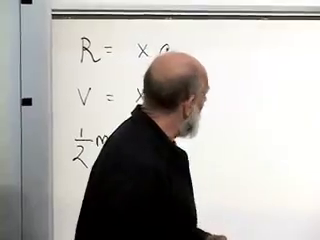
\includegraphics[width=0.72\textwidth]{lecture_09_figure_02.png}
  \caption{平直膨脹度規，標度因子乘上歐幾里得空間線元。來源畫面時間：00:09:12。}
  \label{fig:l09-expanding-metric-board}
\end{figure}

想像座標標記畫在一張橡膠片上。標記始終附著在橡膠片上，但標記之間的物理距離會逐漸增大。因此，像「從\(x=0\)到\(x=1\)」這樣的座標差只是一對標籤；這段間隔所代表的距離是\(a(t)\)。找出支配這個標度因子的方程，就是本講座要探討的動力學問題。

\section{閉合、平直與開放的空間幾何}

平直性是觀測上的簡化，並非均勻性的必然結果。均勻且各向同性的空間幾何有三種：正曲率、零曲率和負曲率。要理解正曲率的情形，必須仔細區分維度。

軌跡
\begin{equation}
  X_1^2+X_2^2=R^2
\end{equation}
是一個圓，也就是一維球面\(S^1\)。它所包圍的內部是圓盤，也稱為二維球。增加一個嵌入座標，就得到
\begin{equation}
  X_1^2+X_2^2+X_3^2=R^2,
\end{equation}
普通的二維球面\(S^2\)。再增加第四個嵌入座標，就得到
\begin{equation}
  X_1^2+X_2^2+X_3^2+X_4^2=R^2,
  \label{eq:l09-three-sphere}
\end{equation}
三維球面\(S^3\)；它本身是三維空間。我們無法想像它嵌入四維空間的樣子，但其內在幾何並不需要這種嵌入才能存在。

\begin{figure}[H]
  \centering
  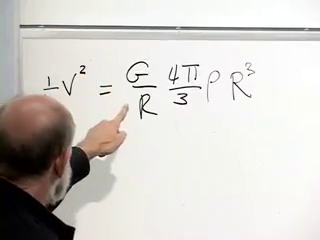
\includegraphics[width=0.72\textwidth]{lecture_09_figure_03.png}
  \caption{用來引介三維球面的嵌入方程。來源畫面時間：00:16:40。}
  \label{fig:l09-three-sphere-board}
\end{figure}

理想球面上的每一點在幾何上都與其他點等價，而每一點上的各個方向也都等價。因此，球面既均勻又各向同性。如果半徑乘上\(a(t)\)，整個空間便會膨脹或收縮，卻不會在球面上選出某個中心。將這樣的宇宙往回追溯，並不會把所有物質都放到外部虛空中的某個特殊位置。整個空間都會縮小，因此任意兩點都會彼此接近。大爆炸並不是從空間中的某一點向外爆炸。

在正曲率球面上，測地三角形的內角和大於
\(180^\circ\)。平直三角形的內角和恰好等於\(180^\circ\)。在均勻的負曲率幾何中，內角和小於\(180^\circ\)；馬鞍面只是對這種幾何不完全準確的示意。這些內在幾何檢驗可以區分這三種情形。

\begin{figure}[H]
  \centering
  \includegraphics[width=0.72\textwidth]{lecture_09_figure_07.png}
  \caption{以各自特有的三角形形狀示意正曲率、零曲率與負曲率。來源畫面時間：00:37:30。}
  \label{fig:l09-curvature-board}
\end{figure}

局部度規完全平直，本身並不能證明空間在拓撲上是無限的。數學上也可能存在緊緻的平直拓撲，不過本講座採用最簡單的無限歐幾里得模型。
\editorialnote{這項關於整體拓撲的限定，對後續任何局部動力學都沒有必要。}

\section{共動標籤與哈伯定律}

現在回到膨脹的平直薄片，在上面畫出座標網格。在共動座標中，網格隨著大尺度物質流一起膨脹。星系，或更精確地說，足夠粗粒化後的星系團，會維持近似固定的座標標籤，即使它與另一個共動物體之間的物理距離正在改變。

\begin{figure}[H]
  \centering
  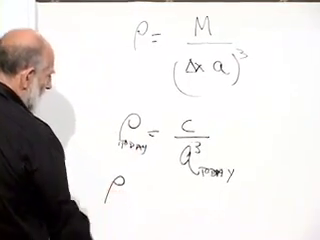
\includegraphics[width=0.72\textwidth]{lecture_09_figure_04.png}
  \caption{隨膨脹的空間薄片一起伸展的座標網格。來源畫面時間：00:22:20。}
  \label{fig:l09-comoving-grid-board}
\end{figure}

兩個物體沿\(x\)軸相隔固定的共動間隔\(\Delta x\)，其物理距離為
\begin{equation}
  D(t)=a(t)\,\Delta x.
  \label{eq:l09-physical-distance}
\end{equation}
保持\(\Delta x\)不變並對時間微分，得到
\begin{equation}
  v(t)=\dot a(t)\,\Delta x
      =\frac{\dot a(t)}{a(t)}D(t).
\end{equation}
定義
\begin{equation}
  H(t)\equiv\frac{\dot a(t)}{a(t)},
  \label{eq:l09-hubble-parameter}
\end{equation}
便得到哈伯定律：
\begin{equation}
  v=H(t)D.
  \label{eq:l09-hubble-law}
\end{equation}
「哈伯常數」中的「常數」，是指在指定的宇宙時刻，這個量在空間各處都相同；這不表示它在整個宇宙歷史中保持不變。

\begin{figure}[H]
  \centering
  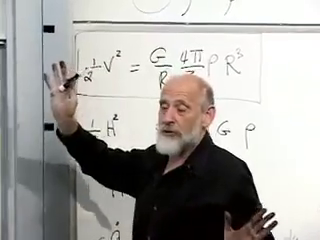
\includegraphics[width=0.72\textwidth]{lecture_09_figure_05.png}
  \caption{黑板上的推導：\(D=a\Delta x\)，
  \(v=(\dot a/a)D=HD\)。來源畫面時間：00:26:40。}
  \label{fig:l09-hubble-board}
\end{figure}

\begin{classroomqa}
\audiencequestion{如果我們看到一個遙遠星系的時間較早，推得的哈伯參數真的應該等於今天在附近測得的值嗎？}
\lecturerresponse{只有當回溯時間相較於宇宙年齡很短時，才是如此。在不太遠的距離上，\(H(t)\)的變化不大，因此用單一數值仍然合適。到了真正的宇宙學距離，我們看到的是較早的宇宙時期，就必須納入\(a\)和\(H\)隨時間變化的影響。這也是我們需要標度因子動力學方程的原因之一。}
\end{classroomqa}

\section{膨脹座標系中的零測地線}

\begin{classroomqa}
\audiencequestion{標度因子會影響光在遙遠星系之間的傳播嗎？}
\lecturerresponse{光線沿著零測地線傳播，因此\(d\tau=0\)。對於沿正\(x\)軸傳播的光線，\(dy=dz=0\)，膨脹度規給出
\begin{align}
  0&=dt^2-a^2(t)dx^2,
  &dt&=a(t)dx,\notag\\
  &&\frac{dx}{dt}&=\frac{1}{a(t)}.
  \label{eq:l09-null-ray}
\end{align}
隨著\(a(t)\)增大，座標速度會降低，但光的局部物理速度仍為\(c=1\)。固定的座標間隔所代表的物理距離則會逐漸增加。}
\end{classroomqa}

\begin{figure}[H]
  \centering
  \includegraphics[width=0.72\textwidth]{lecture_09_figure_06.png}
  \caption{徑向光傳播的零條件與\(dt=a(t)dx\)。來源畫面時間：00:30:54。}
  \label{fig:l09-null-board}
\end{figure}

我們可以選擇一套座標，讓同一件事聽起來像是「光在較遠處變慢了」，但相應地，長度和時鐘的描述也會變得彆扭。以空間膨脹來描述更簡潔，因為這保留了局部的陳述：每位自由落下的觀測者測得的光速都相同。

\begin{classroomqa}
\audiencequestion{有證據顯示，遙遠星系中的局部光傳播和原子物理與我們這裡相同嗎？}
\lecturerresponse{只有無量綱的比較才具有可操作的意義。選定一種原子尺度作為長度單位，再選定原子或核子的週期作為時間單位，接著詢問光穿越所選長度需要多少個這樣的週期。光譜觀測支持這項說法：這些無量綱比值在遙遠區域也相同。證據雖然是間接的，但這正是檢驗局部定律是否一致的一類比較。}
\end{classroomqa}

當可觀測宇宙極其微小時，光可以在相應的光穿越時間內迅速穿過一個給定的物理區域。這並不表示\(c\)有所不同，而是表示該區域本身很小。

\section{宇宙中的牛頓球體}

現在我們從運動學轉向動力學。以我們所在的位置為原點，畫出一個足以容納許多星系和星系團的大球，並在球面上選取一個星系。在均勻宇宙中，質量分布以我們為中心呈球對稱；牛頓殼層定理給出兩個關鍵事實：
\begin{enumerate}
  \item 所選半徑以外的球對稱物質，對球面上的星系施加的牛頓合力為零；
  \item 球內所有物質對這種徑向運動的作用，都等同於集中在球心。
\end{enumerate}
我們採用一個自身靜止的參考系，因此以下論證中的速度和加速度都是相對於我們測量的。

\begin{figure}[H]
  \centering
  \includegraphics[width=0.72\textwidth]{lecture_09_figure_08.png}
  \caption{殼層定理的構造：我們位於中心，測試星系位於大型均勻球體的邊界。來源畫面時間：00:41:10。}
  \label{fig:l09-shell-board}
\end{figure}

\begin{figure}[H]
  \centering
  \begin{tikzpicture}[scale=0.92,>=Latex]
    \draw[thick] (0,0) circle (2.35);
    \fill (0,0) circle (2pt) node[below left] {us};
    \fill (2.35,0) circle (2.2pt) node[right] {test galaxy \(m\)};
    \draw[->,thick,blue!65!black] (0.18,0) -- (2.15,0)
      node[midway,above] {\(R=a(t)x\)};
    \draw[->,thick,red!65!black] (2.35,0.12) -- (3.25,0.12)
      node[midway,above] {\(v=\dot a(t)x\)};
    \node[align=center,text width=7cm] at (0,-2.85)
      {outside shells cancel;\\enclosed mass acts at the center};
  \end{tikzpicture}
  \caption{牛頓構造的清晰重繪。}
  \label{fig:l09-shell-clean}
\end{figure}

若星系的共動座標\(x\)固定，則其物理半徑和速度為
\begin{equation}
  R(t)=x a(t),
  \qquad
  v(t)=x\dot a(t)=H(t)R(t).
  \label{eq:l09-radius-velocity}
\end{equation}
令\(M\)為球體所包圍的質量，\(m\)為測試星系的質量。牛頓能量為
\begin{equation}
  E=\frac12 m v^2-\frac{GMm}{R}.
  \label{eq:l09-newtonian-energy}
\end{equation}

\begin{figure}[H]
  \centering
  \includegraphics[width=0.72\textwidth]{lecture_09_figure_09.png}
  \caption{完整的板書推導：\(R=xa\)、\(v=x\dot a\)，以及針對\(E=0\)的牛頓能量方程。來源畫面時間：00:48:40。}
  \label{fig:l09-energy-board}
\end{figure}

能量可以是正、零或負。我們先從逃逸與再坍縮之間的邊界情形\(E=0\)開始，此時
\begin{equation}
  \frac12 v^2=\frac{GM}{R}.
  \label{eq:l09-zero-energy}
\end{equation}

\begin{classroomqa}
\audiencequestion{退行星系的總能量為零，代表什麼？}
\lecturerresponse{這正是達到逃逸速度的情形。正能量表示速度高於逃逸速度；負能量表示速度低於逃逸速度，在只有物質的牛頓圖像中，星系最終會返回。我們先從兩種可能性之間的邊界推導，得到平直方程後再回頭討論另外兩種能量符號。}
\end{classroomqa}

\begin{classroomqa}
\audiencequestion{球體膨脹時，所包圍的質量\(M\)會改變嗎？}
\lecturerresponse{不會。球體是共動的，因此相同的粒子會一直留在其中。球體的物理體積增大，密度下降，但所包圍的總質量不變。\(M\)與\(\rho(t)\)的區別至關重要。}
\end{classroomqa}

對於均勻密度\(\rho(t)\)，
\begin{equation}
  M=\frac{4\pi}{3}\rho(t)R^3.
  \label{eq:l09-enclosed-mass}
\end{equation}
代入\eqref{eq:l09-zero-energy}，得到
\begin{equation}
  \frac12 v^2
  =\frac{G}{R}\left(\frac{4\pi}{3}\rho R^3\right).
  \label{eq:l09-enclosed-energy}
\end{equation}

\begin{figure}[H]
  \centering
  \includegraphics[width=0.72\textwidth]{lecture_09_figure_10.png}
  \caption{將所包圍質量代入零能量方程。來源畫面時間：00:54:16.060。}
  \label{fig:l09-enclosed-mass-board}
\end{figure}

利用\(v=HR\)，得到
\begin{align}
  \frac12 H^2R^2
    &=\frac{4\pi G}{3}\rho R^2,\\
  H^2
    &=\frac{8\pi G}{3}\rho.
\end{align}
因此，零能量、空間平直的膨脹定律為
\begin{equation}
  \boxed{\left(\frac{\dot a}{a}\right)^2
  =\frac{8\pi G}{3}\rho(t)}.
  \label{eq:l09-flat-friedmann}
\end{equation}
消去\(R^2\)並非偶然。無論選哪個共動星系作為測試物體，均勻宇宙都必須給出相同的\(H(t)\)。

\begin{figure}[H]
  \centering
  \includegraphics[width=0.72\textwidth]{lecture_09_figure_11.png}
  \caption{板書展示了半徑的消去，以及由此得到的平直弗里德曼關係。來源畫面時間：00:57:30。}
  \label{fig:l09-friedmann-board}
\end{figure}

\begin{classroomqa}
\audiencequestion{有證據支持零能量關係嗎？}
\lecturerresponse{等式兩邊都可以由觀測推得：\(H\)來自退行資料，而\(\rho\)則是將恆星、氣體、暗物質和真空能都納入計算後得到的。講座當時的比較顯示，兩邊在約百分之幾的精度內一致。這項限定很重要：必須計入所有形式的能量，而且後面對真空能的討論會修正對逃逸速度的直觀解讀。}
\end{classroomqa}

在\(c=1\)的單位制下，質量密度和能量密度的單位相同。因此，符號\(\rho\)將表示所討論組分對應的總能量密度。

\section{普通物質與三分之二次方定律}

在知道\(\rho(t)\)如何變化之前，方程\eqref{eq:l09-flat-friedmann}還不是封閉的。先用緩慢運動的非相對論粒子填滿一個共動長方體。它的座標尺寸固定，物理體積則按下式增大：
\begin{equation}
  V(t)=a^3(t)\,\Delta x\,\Delta y\,\Delta z.
\end{equation}
盒中的粒子數和靜止質量維持不變，因此
\begin{equation}
  \rho_{\mathrm m}(t)=\frac{C_{\mathrm m}}{a^3(t)}.
  \label{eq:l09-matter-dilution}
\end{equation}
以目前時期\(t_0\)為基準正規化，得到
\begin{equation}
  \frac{\rho_{\mathrm m}(t)}{\rho_{\mathrm m,0}}
  =\left(\frac{a_0}{a(t)}\right)^3.
  \label{eq:l09-matter-normalized}
\end{equation}

\begin{figure}[H]
  \centering
  \includegraphics[width=0.72\textwidth]{lecture_09_figure_12.png}
  \caption{物質密度按\(a^{-3}\)稀釋，以及以現在為基準的正規化。來源畫面時間：01:04:47.940。}
  \label{fig:l09-density-board}
\end{figure}

\begin{classroomqa}
\audiencequestion{目前宇宙的能量密度大約是多少？只靠普通原子能提供這麼多能量嗎？}
\lecturerresponse{只計算可見的重子物質，並不足以回答這個問題。暗物質和暗能量也必須以等效質能計入。講座引用的粗略範圍是每立方公尺相當於一個原子至數十個氫原子的質量，強調的是數量級，而非精確盤點。}
\end{classroomqa}

將\eqref{eq:l09-matter-dilution}代入\eqref{eq:l09-flat-friedmann}，並把所有與時間無關的因子吸收到一個正的常數\(C\)中：
\begin{equation}
  \left(\frac{\dot a}{a}\right)^2=\frac{C}{a^3},
  \qquad
  \dot a^2=\frac{C}{a}.
  \label{eq:l09-matter-ode}
\end{equation}
求解有兩種直接的方法。假設冪律形式\(a=K t^p\)，便須滿足
\begin{equation}
  p-1=-\frac{p}{2},
  \qquad p=\frac23.
\end{equation}
另一種等價的做法是取膨脹解的平方根分支並積分：
\begin{equation}
  a^{1/2}\frac{da}{dt}=\sqrt C,
  \qquad
  \int a^{1/2}da=\sqrt C\int dt,
\end{equation}
因此，選定大爆炸時刻為時間原點後，
\begin{equation}
  a^{3/2}\propto t,
  \qquad
  \boxed{a(t)\propto t^{2/3}}.
  \label{eq:l09-matter-solution}
\end{equation}
現場推導在配對係數時一度漏掉一個因子，之後回到積分重新檢查指數。筆記保留了這項檢查，但只列出修正後的代數推導。

\begin{figure}[H]
  \centering
  \includegraphics[width=0.72\textwidth]{lecture_09_figure_13.png}
  \caption{冪律假設與框出的指數\(p=2/3\)。來源畫面時間：01:13:05。}
  \label{fig:l09-matter-solution-board}
\end{figure}

對解微分，得到
\begin{equation}
  H(t)=\frac{\dot a}{a}=\frac{2}{3t}.
  \label{eq:l09-matter-hubble}
\end{equation}
過去的哈伯參數較大。因此，當觀測距離遠到足以涵蓋明顯的回溯時間時，不應把今天的\(H_0\)當成不變的數值，直接外推局部線性關係。

\begin{figure}[H]
  \centering
  \includegraphics[width=0.72\textwidth]{lecture_09_figure_14.png}
  \caption{將\(\dot a/a\)代入\(a\propto t^{2/3}\)，得到
  \(H=2/(3t)\)。來源畫面時間：01:20:42。}
  \label{fig:l09-hubble-time-board}
\end{figure}

\section{能量符號與空間曲率}

牛頓式推理帶領我們推導出平直、零能量的情形。廣義相對論還補充了一項僅靠殼層定理無法得到的事實：牛頓式比能量的正負，對應於空間曲率的正負。
\begin{center}
\begin{tabular}{@{}>{\raggedright\arraybackslash}p{0.20\linewidth}
                    >{\raggedright\arraybackslash}p{0.29\linewidth}
                    >{\raggedright\arraybackslash}p{0.37\linewidth}@{}}
  \toprule
  總能量&空間曲率&僅含物質時的演化\\
  \midrule
  正&負（開放）&永遠膨脹\\
  零&零（平直）&漸近於逃逸邊界\\
  負&正（閉合）&膨脹、轉向、再坍縮\\
  \bottomrule
\end{tabular}
\end{center}
最後一欄假設沒有真空能。在拋射體的類比中，正能量表示速度高於逃逸速度，零能量表示速度恰好等於逃逸速度，負能量則表示速度低於逃逸速度。愛因斯坦方程分別將這三種情形對應到開放、平直和閉合的空間幾何。

\section{光子與二分之一次方定律}

物質定律\(\rho\propto a^{-3}\)假設每個粒子的能量近似固定，而數密度逐漸下降。光子不符合這項假設。對光子而言，
\begin{equation}
  E=h\nu=\frac{hc}{\lambda}.
\end{equation}
宇宙膨脹會使波長按標度因子的比例伸長，
\begin{equation}
  \lambda\propto a,
  \qquad E\propto a^{-1}.
\end{equation}
光子數密度仍按\(a^{-3}\)下降，而每個光子的能量還會額外帶來一個\(a^{-1}\)因子。因此
\begin{equation}
  \boxed{\rho_{\mathrm r}(t)\propto a^{-4}(t)}.
  \label{eq:l09-radiation-dilution}
\end{equation}

吉他弦的類比呈現了這個物理圖像。先撥動琴弦，再拉長它振動的部分：波長變長，音調降低。膨脹共動盒中的光子模式也有類似的行為。反過來看，壓縮會縮短波長並提高光子能量。

\begin{figure}[H]
  \centering
  \includegraphics[width=0.72\textwidth]{lecture_09_figure_15.png}
  \caption{黑板上將物質密度關係推展至輻射的標度關係\(\rho_{\mathrm r}\propto a^{-4}\)。來源畫面時間：01:29:20。}
  \label{fig:l09-radiation-board}
\end{figure}

將\(\rho_{\mathrm r}\propto a^{-4}\)代入平直弗里德曼方程，得到
\begin{equation}
  \left(\frac{\dot a}{a}\right)^2=\frac{C_{\mathrm r}}{a^4},
  \qquad
  \dot a\propto a^{-1},
\end{equation}
因此
\begin{equation}
  \boxed{a(t)\propto t^{1/2}}.
  \label{eq:l09-radiation-solution}
\end{equation}
這比\(t^{2/3}\)的增長慢。回溯到足夠早的時期，輻射必定會主導普通物質，因為當\(a\)減小時，\(a^{-4}\)上升的速度比\(a^{-3}\)快。講座將物質與輻射的交會時期定在標度因子約比今天小一千倍的時候。在交會之前，宇宙由輻射主導；交會之後，則由物質主導了很長一段時間。

\section{真空能與指數膨脹}

真空能的標度行為正好相反。真空能密度是空無一物的空間所具有的性質，不會隨宇宙膨脹而稀釋：
\begin{equation}
  \rho_\Lambda=\text{constant}.
  \label{eq:l09-vacuum-density}
\end{equation}
普通物質和輻射在過去的密度較高，這一項則不會。因此，在早期宇宙中，真空能較不重要；隨著其他組分稀釋，它便愈來愈重要。講座採用當時的估計，認為真空能約占今日宇宙能量密度的\(70\%\)。

當\(\rho_\Lambda\)為常數時，方程\eqref{eq:l09-flat-friedmann}給出固定的膨脹率
\begin{equation}
  H_\Lambda=\sqrt{\frac{8\pi G}{3}\rho_\Lambda},
  \qquad
  \frac{\dot a}{a}=H_\Lambda.
\end{equation}
因此
\begin{equation}
  \boxed{a(t)=a(t_i)e^{H_\Lambda(t-t_i)}}.
  \label{eq:l09-vacuum-solution}
\end{equation}

\begin{figure}[H]
  \centering
  \includegraphics[width=0.72\textwidth]{lecture_09_figure_16.png}
  \caption{導出指數膨脹的定密度方程。來源畫面時間：01:35:48。}
  \label{fig:l09-vacuum-board}
\end{figure}

以講座引用的觀測尺度來看，宇宙的線性尺度約每一百億至一百二十億年加倍。這個微小但非零的真空能密度為何存在，至今仍無法解釋；它的存在及其對膨脹的影響則是經驗事實。

\begin{classroomqa}
\audiencequestion{在這段討論中，真空能和暗能量是同一回事嗎？}
\lecturerresponse{是的。這裡的「暗能量」指密度固定的真空能，等價於宇宙學常數。也可以設想更一般、隨時間變化的暗能量模型，但這些模型不在本講座的計算範圍內。}
\end{classroomqa}

\section{膨脹宇宙如何使光紅移}

\begin{classroomqa}
\audiencequestion{光子怎麼會知道我們選了膨脹的共動座標，因而降低自己的能量？}
\lecturerresponse{光子並不會對我們的標記作出反應。它們是在物理間隔不斷變化的幾何中傳播。若一列波佔據的區域，其物理尺度加倍，波長也會加倍。共動座標只是方便地描述這種伸長，並不會造成伸長。}
\end{classroomqa}

\begin{classroomqa}
\audiencequestion{今天抵達我們的背景光子來自何處？}
\lecturerresponse{看得愈遠，就看得愈早。最後，我們會看到宇宙物質處於電離電漿的時期；當時自由帶電粒子不斷散射光子，因此電漿是不透明的。光子最後一次能不受阻礙地傳到我們這裡的邊界，在觀測者周圍呈現為一個球面，稱為最後散射面。}
\end{classroomqa}

\begin{figure}[H]
  \centering
  \includegraphics[width=0.72\textwidth]{lecture_09_figure_17.png}
  \caption{以觀測者為中心的最後散射面，以及一層層愈來愈遠的殼層示意圖。來源畫面時間：01:42:05。}
  \label{fig:l09-last-scattering-board}
\end{figure}

\begin{figure}[H]
  \centering
  \begin{tikzpicture}[scale=0.9,>=Latex]
    \fill (0,0) circle (2pt) node[below] {observer};
    \draw[thick,orange!70!black] (0,0) circle (2.55);
    \node[orange!70!black,align=center] at (0,3.05)
      {surface of last scattering};
    \foreach \a in {25,75,145,210,285,335}{
      \draw[->,blue!60!black] ({2.55*cos(\a)},{2.55*sin(\a)}) --
        ({1.7*cos(\a)},{1.7*sin(\a)});
    }
    \draw[decorate,decoration={snake,amplitude=1.5pt,segment length=7pt},
      red!65!black,thick,->] (-2.5,0) -- (-0.15,0);
    \node[red!65!black,below] at (-1.35,-0.15)
      {redshifted photon};
  \end{tikzpicture}
  \caption{最後散射圖像的清晰重繪。}
  \label{fig:l09-last-scattering-clean}
\end{figure}

這些輻射發射時具有熱電漿的特徵光譜；抵達我們時，波長約增加了一千倍。用講座中的多普勒說法來描述，遙遠的發射面快速遠離，其輻射受到強烈紅移。用幾何說法來描述，波在傳播過程中被拉長。兩種圖像描述的是同一關係：
\begin{equation}
  1+z=\frac{\lambda_0}{\lambda_{\mathrm{em}}}
      =\frac{a_0}{a_{\mathrm{em}}}.
  \label{eq:l09-cosmological-redshift}
\end{equation}
\editorialnote{方程\eqref{eq:l09-cosmological-redshift}是講座中拉伸與多普勒描述的標準定量形式。}

若在較早的宇宙時期觀測，依照相應的圖像，最後散射面會比較近；觀測到的背景光子紅移也較小，因此能量較高。隨著宇宙時間推進，從早期電漿傳到共動觀測者的光子，其波長會逐漸變長。

\section{紅移後的光子能量去了哪裡？}

\begin{classroomqa}
\audiencequestion{光子發射時的能量是\(h\nu_{\mathrm{em}}\)，抵達時已紅移，能量也減少了。減少的能量去了哪裡？}
\lecturerresponse{牛頓推導一開始就是能量方程。其宇宙學形式將膨脹率與物質能量密度聯繫起來，因此不能把物質能量和膨脹視為各自守恆的帳目。講座將光子流失的能量描述為納入膨脹的動能帳目。以充滿輻射的活塞為例，這個類比就很具體：輻射壓將活塞向外推，光子的波長隨之增加，流失的能量則轉化為機械功和活塞的動能。}
\end{classroomqa}

\begin{figure}[H]
  \centering
  \includegraphics[width=0.72\textwidth]{lecture_09_figure_18.png}
  \caption{黑板上將框起來的牛頓能量方程置於相應的弗里德曼方程上方。來源畫面時間：01:44:42。}
  \label{fig:l09-energy-bookkeeping-board}
\end{figure}

\begin{classroomqa}
\audiencequestion{是什麼讓輻射能量與膨脹耦合？}
\lecturerresponse{壓力。在裝有可移動活塞的圓筒中，光子會把動量傳給壁面。活塞移動時，輻射便做功；光子的波長增加，能量則降低。均勻膨脹的宇宙並沒有字面意義上的外部活塞，但\(p\,dV\)類比說明了為何輻射能量密度的下降速度，會快於單靠粒子數稀釋所造成的下降。}
\end{classroomqa}

\begin{figure}[H]
  \centering
  \includegraphics[width=0.72\textwidth]{lecture_09_figure_19.png}
  \caption{用來呈現壓力做功的可移動光子活塞。來源畫面時間：01:46:40。}
  \label{fig:l09-piston-board}
\end{figure}

\begin{figure}[H]
  \centering
  \begin{tikzpicture}[scale=0.92,>=Latex]
    \draw[thick] (0,0) rectangle (5.3,2.6);
    \draw[very thick] (4.25,0) -- (4.25,2.6);
    \draw[very thick] (4.25,1.3) -- (5.25,1.3);
    \draw[->,thick,red!65!black] (5.25,1.3) -- (6.2,1.3)
      node[right] {moving piston};
    \foreach \y in {0.55,1.3,2.05}{
      \draw[decorate,decoration={snake,amplitude=1.4pt,segment length=6pt},
        blue!65!black,->] (0.35,\y) -- (3.9,\y);
    }
    \node at (2.15,-0.45) {radiation does \(p\,dV\) work};
  \end{tikzpicture}
  \caption{輻射與活塞類比的清晰重繪。}
  \label{fig:l09-piston-clean}
\end{figure}

廣義相對論中的能量需要謹慎處理。在一般的膨脹時空中，未必存在唯一的守恆全域能量，可與孤立牛頓系統的能量相類比。局域的應力—能量守恆仍然成立；對均勻流體而言，它導出連續性方程
\begin{equation}
  \dot\rho+3H(\rho+p)=0,
  \label{eq:l09-continuity}
\end{equation}
其中包含壓力做功項，這正是物質與輻射標度律的由來。\editorialnote{方程 \eqref{eq:l09-continuity} 是局域廣義相對論的精確表述，也是講座中刻意採用牛頓式能量收支類比的依據。}

真空能使這個問題格外尖銳。由於其密度保持不變而體積持續增大，共動區域內的真空能總量便會增加。真空能的負壓是引力源的一部分，並會驅動加速膨脹。因此，若不把幾何與壓力做功納入考量，就不應要求樸素理解下「共動盒中的物質能量」單獨守恆。

\section{為什麼時間項中的標度因子可以消去}

\begin{classroomqa}
\audiencequestion{為什麼標度因子乘在度規的空間部分上，卻沒有乘在時間部分上？}
\lecturerresponse{這是時間座標的選擇。假設一開始採用共形時間座標 \(t\)，度規為
\begin{equation}
  d\tau^2=A^2(t)\left(dt^2-dx^2\right).
\end{equation}
再以下式定義新的宇宙時間 \(T\)：
\begin{equation}
  dT=A(t)\,dt.
\end{equation}
則有
\begin{equation}
  d\tau^2=dT^2-A^2\bigl(t(T)\bigr)dx^2.
\end{equation}
時間微分前的共同因子便消去了，而物理標度因子仍留在空間項中。}
\end{classroomqa}

\begin{figure}[H]
  \centering
  \includegraphics[width=0.72\textwidth]{lecture_09_figure_20.png}
  \caption{將共形時間轉換為宇宙時間的時間座標重新定義 \(dT=A(t)dt\)。來源影格時間為 01：51：05。}
  \label{fig:l09-time-reparam-board}
\end{figure}

\section{曲率、真空能與宇宙的命運}

\begin{classroomqa}
\audiencequestion{如果宇宙具有正曲率，我們現在應該已經看到星系朝我們移動嗎？}
\lecturerresponse{未必。以低於逃逸速度發射的拋射體會先向外運動，到達轉折點後才落回。我們觀測到的宇宙正處於膨脹階段。若沒有真空能，正曲率的物質宇宙最終會再坍縮。若正值真空能足夠大，就能阻止宇宙在轉折點折返；觀測到的真空能值似乎大到足以使宇宙長期持續指數式膨脹，即使空間曲率很小也是如此。}
\end{classroomqa}

指數式膨脹的未來並非能量天堂。恆星終將燃盡，物質與輻射的密度會呈指數式下降，遙遠區域也會超出彼此的因果聯繫範圍。真空能依然存在，而一般結構則會逐漸變得更冷、更稀薄。

\begin{classroomqa}
\audiencequestion{愈往過去追溯，光子會比一般粒子更多嗎？}
\lecturerresponse{光子數與重子數之比早已極大；依照講座中的估計，每個重子約有 \(10^{10}\) 個光子，而共動體積內的這兩種粒子數都近似保持不變。往過去追溯時，主要改變的是每個光子的能量。光子能量會按 \(a^{-1}\) 增加，非相對論性粒子的靜止質量則不會。因此，即使粒子數之比本身未必改變，輻射在早期仍會主導能量密度。}
\end{classroomqa}

核心教訓是，單靠幾何並不能決定宇宙的演化歷史。平坦的弗里德曼方程給出膨脹與能量密度之間的關係，而物質成分則決定它們如何隨時間變化。非相對論性物質使 \(a\propto t^{2/3}\)，輻射使 \(a\propto t^{1/2}\)，恆定的真空能則導致指數式膨脹。這三條定律勾勒出宇宙各個相繼的時代，也說明了為什麼同一個標度因子會支配距離、紅移與哈勃參數的變化。
